\subsection{Gestion de version}\label{subsec:gestion-de-version}

La gestion de version, ou versioning, est une pratique essentielle dans tout projet de développement.
Pour ce projet, nous avons utilisé Git comme système de gestion de versions et GitHub pour héberger notre code source.

Au départ du projet, j'ai choisi d'utiliser une seule branche pendant la majeure partie de la première phase.
Cette approche était suffisante pour répondre aux besoins du projet à ce stade, permettant de maintenir une simplicité de gestion.

Cependant, une fois le projet publié sur DockerHub et la mise en place du CI/CD, il est devenu évident que l'utilisation d'une seule branche n'était plus la meilleure option.
J'ai alors créé une branche de développement distincte.
Cette branche a permis de tester et de sauvegarder le code sans perturber la version en production.

Pour la rédaction de ce rapport, j'ai également créé une branche spécifique.
Cette approche a permis de travailler sur le rapport sans interférer avec le code de l'application.

Pour la gestion de l'infrastructure du projet, un second repository GitHub a été utilisé.
Ce choix a été motivé par le fait que l'infrastructure du projet était basée sur un autre projet existant que j'ai forké.
Ce repo distinct pour l'infrastructure a permis de maintenir une séparation claire entre le code de l'application et la gestion de l'infrastructure.

\subsection{Intégration et déploiement continu (CI/CD)}\label{subsec:integration-et-deploiement-continu-(ci/cd)}

Pour l'intégration continue (CI), j'ai mis en place des tests automatisés sur une grande partie des composants du backend et du frontend.

\begin{figure}[H]
    \begin{minipage}[b]{0.5\textwidth}
        \centering
        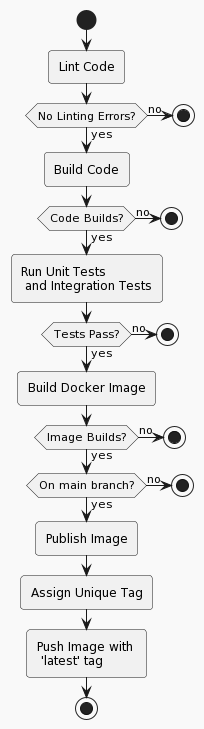
\includegraphics[height=0.3\textheight, keepaspectratio]{images/ci_workflow}
        \caption{Workflow d'intégration continue}
        \label{fig:ci_workflow}
    \end{minipage}%
    \begin{minipage}[b]{0.5\textwidth}
        Le workflow de CI est le suivant :

        \begin{itemize}
            \item Lint du code : vérification des erreurs de syntaxe.
            \item Build du code : si aucune erreur de linting n'est détectée, je peux construire le code.
            \item Tests unitaires et d'intégration : si le code se construit correctement, je lance les tests.
            \item Construction de l'image Docker : si les tests passent, je construis l'image du conteneur.
            \item Publication de l'image : si la construction de l'image réussit, je la publie sur DockerHub (seulement si je suis sur la branche principale).
        \end{itemize}
    \end{minipage}
\end{figure}

Pour le déploiement continu (CD), j'utilise un conteneur Watchtower qui, via le socket Docker,
vérifie régulièrement quelle version du conteneur est utilisée et si elle correspond bien à celle demandée.
Watchtower vérifie également la signature du conteneur en plus de son tag,
ce qui lui permet de mettre à jour un conteneur avec le tag "latest" lorsque l'image change.
Watchtower compare régulièrement la version courante des conteneurs contre celle hébergée sur DockerHub et si elles ne correspondent pas,
alors le conteneur est mis à jour.

\subsection{Conclusion}\label{subsec:conclusion}

La gestion de version a été un aspect crucial de ce projet.
L'adoption d'une approche adaptative, passant d'une seule branche à plusieurs branches en fonction des besoins du projet, a prouvé son efficacité.
De même, l'implémentation des pratiques de CI/CD a grandement amélioré le flux de travail et la qualité de
l'application, rendant le processus de développement plus fluide et fiable.